\documentclass[11pt,letterpaper]{article}
\usepackage[margin=.83in,top=.78in,bottom=.76in,headheight=14pt,headsep=15pt]{geometry}
\usepackage{amsmath,amssymb,booktabs,array,xcolor,tikz,fancyhdr,hyperref}
\usetikzlibrary{arrows.meta,positioning}
\definecolor{ink}{HTML}{183547}\definecolor{pine}{HTML}{126152}
\definecolor{slate}{HTML}{486373}\definecolor{pale}{HTML}{EAF3F0}
\definecolor{rust}{HTML}{9B4C31}\definecolor{blueink}{HTML}{225583}
\hypersetup{colorlinks=true,linkcolor=pine,urlcolor=blueink,pdftitle={Hamiltonian parity in cubic graphs via reflection},pdfauthor={Working manuscript prepared for Dominic Dabish}}
\pagestyle{fancy}\fancyhf{}\fancyhead[L]{\small\sffamily\color{pine} HAMILTONIAN PARITY}\fancyhead[R]{\small\sffamily\color{slate} COMPLEXITY THEORY}
\fancyfoot[L]{\footnotesize\sffamily\color{slate} Working manuscript for Dominic Dabish \enspace / \enspace 21 November 2026}
\fancyfoot[R]{\small\sffamily\color{slate}\thepage}\renewcommand{\headrulewidth}{.35pt}
\renewcommand{\labelitemi}{\(\bullet\)}
\setlength{\parindent}{0pt}\setlength{\parskip}{5.5pt}
\setlength{\abovedisplayskip}{5pt}\setlength{\belowdisplayskip}{5pt}
\setlength{\emergencystretch}{1.5em}
\newcommand{\hd}[1]{\par\medskip{\large\bfseries\color{pine}#1}\par\nobreak}
\newcommand{\lead}[1]{\textbf{\color{ink}#1}\enspace}
\newcommand{\pagehead}[2]{\newpage\phantomsection\pdfbookmark[1]{#1}{#2}{\LARGE\bfseries\color{ink}#1\par}\smallskip}
\newcommand{\boxline}[1]{\par\smallskip\noindent\colorbox{pale}{\parbox{\dimexpr\linewidth-2\fboxsep\relax}{\vspace{4pt}#1\vspace{4pt}}}\par\smallskip}
\newcommand{\hc}{\operatorname{hc}}\newcommand{\sat}{\operatorname{\#SAT}}
\newcommand{\classpar}{\mathord{\oplus}\mathrm P}
\newcommand{\citepaper}[2]{\href{#1}{#2}}
\begin{document}
\phantomsection\pdfbookmark[1]{Main result}{overview}
{\sffamily\small\color{slate} GRAPH THEORY \hfill RESEARCH NOTE}\\[5pt]
{\fontsize{24.88}{30}\selectfont\bfseries\color{ink} Hamiltonian parity in cubic graphs\\[2pt] via reflection\par}
\vspace{3pt}
{\large\color{slate} A two-vertex construction, two colored edges, and the four-clue problem\par}
\medskip
A Hamiltonian cycle visits every vertex once and returns to its starting point. Count a cycle once as an undirected edge set. A cubic graph has three edges at every vertex. Is the number of Hamiltonian cycles odd?

\boxline{\textbf{Main theorem.} This question is $\classpar$-complete on connected simple cubic graphs. Hardness holds when two specified adjacent vertices can be deleted to make the graph bipartite. A Hamiltonian cycle and a proper three-edge-coloring can both be supplied with the graph.}

The class $\classpar$ consists of decision problems asking whether the number of polynomially checkable witnesses is odd. Completeness here is under deterministic polynomial-time many-one reductions. The input graphs in the theorem can be given with their reflection.

\begin{center}
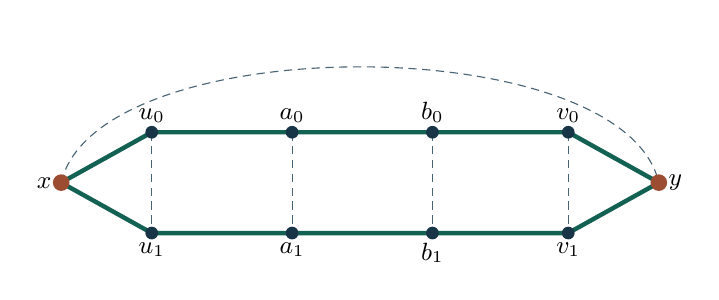
\begin{tikzpicture}[x=1.15cm,y=.8cm, every node/.style={font=\small}]
\coordinate (X) at (-1,0);\coordinate (Y) at (5.6,0);
\foreach \xx/\lab in {0/u,1.55/a,3.1/b,4.6/v}{
 \coordinate (A\lab) at (\xx,.8);\coordinate (B\lab) at (\xx,-.8);
 \draw[slate,densely dashed] (A\lab)--(B\lab);
}
\draw[slate,densely dashed] (X) to[out=77,in=103,looseness=.68] (Y);
\draw[pine,line width=1.6pt] (X)--(Au)--(Aa)--(Ab)--(Av)--(Y)--(Bv)--(Bb)--(Ba)--(Bu)--cycle;
\foreach \lab in {u,a,b,v}{\fill[ink] (A\lab) circle(2.3pt) (B\lab) circle(2.3pt);
 \node[above] at (A\lab) {$\lab_0$};\node[below] at (B\lab) {$\lab_1$};}
\fill[rust] (X) circle(3pt) (Y) circle(3pt);
\node[left] at (X) {$x$};\node[right] at (Y) {$y$};
\end{tikzpicture}\\[3pt]
{\footnotesize\color{slate} The square with edge $uv$ removed becomes the path $u,a,b,v$ on each sheet.}\\[-1pt]
{\footnotesize\color{slate} The solid cycle is fixed by reflection. The two other Hamiltonian cycles exchange places.}
\end{center}
\hd{Why two vertices matter}
Kotzig's theorem gives even total parity on cubic bipartite graphs. The construction above introduces exactly two vertices whose deletion restores bipartiteness. The defect is minimal. On cubic \emph{bipartite} graphs, prescribe different colors on two disjoint edges and ask for the parity of the number of compatible three-edge-colorings. That problem is $\classpar$-complete even when a valid coloring accompanies the graph.

Valiant's 2018 paper listed the complexity of cubic Hamiltonian parity and palette-normalized cubic edge-coloring parity as unresolved. The proof here addresses the two problems on general cubic graphs. It rests on a published parsimonious grid result and a short symmetry argument. Independent peer review and priority are outstanding. P versus NP remains open.

\pagehead{The two-vertex proof}{proof}
\lead{Source.} Let $H$ be a connected simple bipartite graph with all degrees two or three, and choose $e=uv$ with a degree-two endpoint. Every Hamiltonian cycle of $H$ contains $e$. For hardness we take $H$ from the max-degree-three grid problem of the MIT Hardness Group et al.\ (2024, Theorem 18). Its reduction from SAT preserves the number of solutions. A finite nonempty grid graph has a vertex of degree at most two by inspecting an extreme corner. Disconnected inputs and inputs with degree below two have zero Hamiltonian cycles and can be mapped to the explicit even example on page 7.

\lead{Construction of $K$.} Take two copies of $H-e$, indexed by $0$ and $1$. For every vertex $a$ of degree two \emph{in $H$}, add an edge $a_0a_1$, called a rung. Add two vertices $x,y$ and the five edges
\[
     xu_0,\quad xu_1,\quad yv_0,\quad yv_1,\quad xy.
\]
Each old vertex recovers degree three, and each new vertex has degree three. The graph is simple and connected. It has $2|V(H)|+2$ vertices. Interchanging the sheets and fixing $x,y$ gives an involution $\sigma$.

\hd{Which cycles survive modulo two?}
The involution pairs all Hamiltonian cycles not fixed as edge sets. An invariant cycle spans every vertex, so $\sigma$ acts nontrivially on that cycle and fixes $x,y$. A cycle automorphism fixing a vertex either preserves its two traversal directions, in which case it fixes every vertex, or reverses them. Number the vertices starting at $x$ around the cycle of length $2k$. In the second case $\sigma$ sends index $i$ to $-i\bmod 2k$. Its two fixed vertices are opposite, and it fixes no edge even as an unordered pair.

Every rung and the edge $xy$ are fixed as unordered pairs in $K$. Thus an invariant Hamiltonian cycle avoids them all. From $x$ to $y$ it traverses a Hamiltonian $u$--$v$ path in one copy of $H-e$ and returns along its reflected copy. Deleting $x,y$ from the cycle leaves one segment in each sheet, and together they cover all old vertices. Conversely any such path gives exactly one invariant undirected cycle. Adding $e$ closes the path in $H$. Therefore
\[
  \#\{\text{invariant Hamiltonian cycles of }K\}=\hc(H),\qquad
  \hc(K)\equiv\hc(H)\pmod 2.
\]
Membership in $\classpar$ follows by guessing one bit per edge and checking that the selected subgraph is connected with degree two at each vertex.

\lead{Giving away a Hamiltonian cycle.} Add a selector and one free bit to $F$. In the first branch force all original bits to zero and allow the free bit either value. In the other branch require $F$ and set the free bit to zero. Guard each clause by the selector. There are precisely $2+\sat(F)$ models, including two explicit ones. The grid reduction translates either known model to a known cycle, which lifts to an invariant cycle of $K$. Thus total parity stays complete even with a Hamiltonian cycle supplied. Page 4 supplies a coloring as well.

\hd{Sharp distance from bipartiteness}
Delete $x,y$ and use opposite bipartitions on the two sheets. Every surviving edge crosses the parts. A rung at a degree-two endpoint of $e$ forms a triangle with its connector, so $K$ is nonbipartite. In any cubic graph, if deleting a vertex leaves parts $L,R$, the counts $a,b$ of its neighbors in those parts satisfy $a+b=3$ and $a-b=3(|L|-|R|)$. Hence all neighbors lie on one side, which allows the deleted vertex to be restored. A nonbipartite cubic graph therefore needs at least two vertex deletions. The construction attains this minimum. It attains the edge-deletion minimum as well. Assign $x,y$ to opposite parts and delete the single monochromatic edge at each connector. A single edge whose ends lie on the same side after deletion would require $3(|L|-|R|)=\pm2$, which is impossible.

\pagehead{Two colors and four clues}{coloring}
Write $Z(G;p)$ for the number of \emph{labeled} proper edge-colorings of a graph using colors $0,1,2$ subject to clues $p$. A proper coloring at a cubic vertex uses each color exactly once. On two copies of $H$ add a rung between copies of each degree-two vertex, as before, but keep both copies $e_0,e_1$ of $e$. Call this cubic bipartite graph $G$. Prescribe $e_0=0$, $e_1=1$. The edges are disjoint and a rung joins a pair of their endpoints. For a grid source, $G$ is an edge-selected subgraph of a two-layer square lattice.

\hd{A second independent parity argument}
On a coloring of $G$, exchange the sheets and simultaneously exchange colors 0 and 1. The combined involution preserves the two clues. A fixed coloring must assign color 2 to every rung. Its restriction to one sheet consists of a spanning degree-two subgraph $D$ formed by colors 0 and 1. Every degree-two vertex of $H$ uses both of its incident edges, including $e$ at its designated endpoint. The remaining horizontal edges at degree-three vertices have color 2.

Conversely each spanning 2-factor $D$ of $H$ has all cycles even. Its cycle through $e$ has a forced alternation. Each of its other cycles has two choices, and the other sheet is then determined. If $c(D)$ is the number of cycles,
\[
     \#\{\text{fixed colorings}\}
       =\sum_{D\text{ spanning 2-factor of }H}2^{c(D)-1}
       \equiv\hc(H)\pmod2.
\]
Consequently $Z(G;e_0=0,e_1=1)\equiv\hc(K)\pmod2$. With at most one named edge, exchanging the two other colors pairs every full coloring. With two edges fixed to the same color the same pairing applies. The two distinct-colored edges here achieve hardness.

\hd{A four-edge bond preserving the entire count}
Remove $e_0,e_1$. Attach each of the four exposed ends to a different vertex of a new square $K_{2,2}$, choosing the new vertex opposite in bipartition. Color the two new spokes replacing $e_0$ with 0 and the other two with 1. All four spokes are disjoint. On the square, an edge joining vertices with different spoke colors is forced to color 2. Each of the other two edges takes the missing color. Every outside completion therefore has exactly one square extension. With the resulting graph $Q$,
\[
             Z(Q;\text{four spokes})=Z(G;e_0=0,e_1=1).
\]
If $H-e$ is connected, deleting all four spokes leaves two connected components, the square and the outside. Every spoke joins them, so the four spokes form an inclusion-minimal edge cut, or bond. If $H-e$ is disconnected then $H$ has no Hamiltonian cycle. For the hardness reduction replace that input with the even, positive, nonbridge example on page 7. This ensures the bond promise on both answers.

\pagehead{Exact identities and a known solution}{transport}
\lead{Producing a full coloring.} In a connected cubic bipartite graph, if deleting $e_0,e_1$ leaves it connected, there is a perfect matching containing $e_0$ and avoiding $e_1$. To see this, start with fractional weight $1/3$ on every edge. Adding $e_1$ to a path between its ends in the remaining graph gives an even cycle avoiding $e_0$. Perturb alternately by a small positive amount around the cycle, decreasing $e_1$ while leaving $e_0$ unchanged. A fractional perfect matching in a bipartite graph is a convex combination of perfect matchings, so at least one of them contains $e_0$ and omits $e_1$.

Find it by deleting the ends of $e_0$ and forbidding $e_1$, then using bipartite matching and restoring $e_0$. Give it color 0 and alternate colors 1 and 2 on complementary cycles, starting with color 1 at $e_1$. The construction on page 3 transports the coloring to $Q$. Thus the parity hardness holds with a full extension supplied.

\hd{Palette-normalized colorings on the unmarked cubic graph}
Let $U(J)$ count three-edge-colorings up to a global permutation of the palette. In $K$, both $x$ and $y$ see two distinct colors on their edges toward the sheets, and the same third color on $xy$. On cutting out $x,y$, treat their four edges as boundary stubs. For each color the boundary counts on the left and right of the bipartite remainder agree, since that color covers every old vertex once with its boundary stubs included and the two parts have equal size. The bipartitions on the sheets are opposite.

Suppose $xu_0$ has color $a$ and $xu_1$ has color $b$. The stub at $v_1$ is on the same bipartition side as $u_0$ and the stub at $v_0$ is on the same side as $u_1$. Balance and the fact that $yv_0,yv_1$ are distinct force $yv_0=a$ and $yv_1=b$. Relabel $a,b$ as 0 and 1. The two broken edges can now be restored on their respective sheets. This bijection and its inverse give the \emph{integer} equality
\[
                  U(K)=Z(G;e_0=0,e_1=1)=Z(Q;\text{four spokes}).
\]
It also supplies a proper coloring of $K$ in polynomial time on the hardness family. Membership of palette-normalized parity in $\classpar$ follows by fixing the three colors in a prescribed order at one vertex. For an arbitrary cubic $J$, $3U(J)$ is the sum of $2^{c(J-M)-1}$ over perfect matchings $M$ with all complement cycles even. This counts an unordered factorization with one factor distinguished. Reduction modulo two yields $U(J)\equiv\hc(J)$ since only a single spanning even cycle contributes. Every cubic graph has even order.

\hd{Hamiltonian cycles through two specified edges}
Fix any two edges $e,f$ in a cubic bipartite graph $J$. In each palette orbit there is one coloring with $e=0,f=1$ if their colors differ. Orbits with both in the same factor contribute, modulo two, the Hamilton cycles avoiding both, by the matching sum with that factor fixed. Thus $Z(J;e=0,f=1)\equiv\hc(J)+\hc_{\bar e,\bar f}(J)$. By Smith's per-edge evenness, inclusion--exclusion reduces this to $\hc_{e,f}(J)$. Through two disjoint specified edges, Hamiltonian parity is therefore $\classpar$-complete. For two incident edges it is always even by Thomason's Corollary 1.5 and bipartiteness.

\pagehead{Four separating clues and Latin squares}{decision}
\lead{Decision theorem.} In any connected simple cubic bipartite graph, prescribe two red edges and two blue edges. If deleting the four edges disconnects the graph, feasibility and one full coloring can be computed deterministically in polynomial time. This includes placements in which some of the four edges have both ends in the same remaining component. The four clues may touch.

\lead{Proof.} In each remaining component retain a stub of its fixed color at each end of a deleted edge, including both ends of any edge internal to that component. Reject repeated occurrences of one color at one vertex. A possible completion has an internal green perfect matching, hence equally many left and right vertices in the component. For each of red and blue it must then have equally many stubs on the left and right. Check these conditions.

Every component has at least one stub since the original graph was connected. After the balance checks its number of stubs is even. All components together have eight stubs. Thus each component has at most six, and the less frequent color there has zero or two stubs. Choose the more frequent color as the first matching color (ties arbitrary). Its prescribed stubs already cover their vertices. Delete those covered vertices and test for a perfect matching in the remaining internal graph. This test is necessary. If it succeeds, use that matching together with the majority stubs.

In the complement every old vertex has degree two, counting the remaining stubs. With zero minority stubs all components are even cycles. With two, there is a single open path between them and otherwise even cycles. The two stub vertices are on opposite sides. The path, including both stubs, has odd length, so alternating colors gives the same minority color to both boundary edges. This proves sufficiency and constructs a coloring. Glue the components using the fixed original edges. Alternating-path matching gives a simple polynomial implementation.

\lead{The remaining four-clue case.} When deleting the clues leaves the graph connected, removing a red candidate leaves four blue stub ends. Two open paths pair the ends, in addition to even cycles. A completion exists exactly when a red candidate makes \emph{both} paths pair opposite bipartition classes. A polynomial test for that condition on arbitrary connected remainders would finish this four-clue decision classification. The theorem here settles the separating case.

\hd{Two entries in a Latin square encode parity}
For a simple cubic bipartite graph on $n+n$ vertices, identify left vertices with columns and right vertices with symbols. Factor its bipartite complement into $n-3$ perfect matchings and use them as the first $n-3$ complete rows of a labeled Latin square. Each remaining graph edge marks a symbol still available in its column. Assigning its color specifies which of the last three rows receives it. This is an exact bijection between completions and proper edge-colorings.

Consequently the parity of Latin-square completions is $\classpar$-complete with the first $n-3$ rows filled and \emph{just two further entries}, in different rows, columns and symbols, even given a completed square. With one such clue, swapping the other two rows pairs the completions. The four-spoke version gives the same result with four extra entries in two rows. This uses row and column constraints. Transferring this specific threshold to Sudoku would require preserving its block constraints.


\pagehead{An explicit SAT compiler}{cnf}
The grid theorem on page 2 suffices for the complexity classification. The replication package also gives a direct construction from a CNF formula $F$ with $n\ge1$ variables and $L$ literal occurrences to a bipartite graph $H_F$ of degrees two and three. The output of this second construction need not be a grid. It gives
\[
 |V(H_F)|=256L+4n,\qquad
 \#\{\text{spanning 2-factors with one cycle}\}=\sat(F).
\]
An empty clause is replaced by a contradictory pair of unit clauses. Each unused variable is introduced by a tautological clause. $L$ is measured after these changes. Each of the $2^n$ assignments gives precisely one spanning 2-factor. Unsatisfying assignments give three cycles.

\hd{A permutation with one or three cycles}
For a clause $i$ of width $\ell_i$ make parallel lanes $(i,j,b)$ for layers $j=0,\ldots,\ell_i$ and rails $b=0,1$. A central group $i=0$ has as many layers as the widest clause. Write $h_b=(0,0,b)$.
For literal $j$ of clause $i$, swap layers $0$ and $j$ in both groups $0,i$ and on both rails if the literal is true. Execute these conditional swaps in order, interchange groups $0,i$ on layer zero on both rails, then undo the conditional swaps. The net effect exchanges the two groups at the preimage of layer zero. This preimage is zero when the clause fails and the index of the last true literal otherwise.

Execute the clause gadgets in order to obtain a permutation $S$. It sends $h_b$ to itself on a satisfying assignment and to the private zero layer of the first failed clause otherwise. Subsequent clauses leave that private lane untouched. Let $T$ fix $h_1$ and make a single cycle of all remaining lanes. Thus $S^{-1}TS$ has exactly two cycles. Its $h_0,h_1$ lie in different cycles exactly when $F$ is true. Finally apply $(h_0\,h_1)$. A transposition merges different cycles or splits a common cycle. The final permutation therefore has one cycle on a model and three on a nonmodel.

\hd{Realizing every occurrence of a variable coherently}
Group all conditional gates for one variable, using a different port for each occurrence of a lane in the instruction stream. A negative literal uses an unconditional copy of its swap and then a positive-controlled copy. A single even cycle realizes the two complete choices of this variable. Its routing rule and the elimination of private cycles are proved on page 8. Related permutation-program reductions for cycle factors appear in \citepaper{https://arxiv.org/html/2510.18393v2}{H\"orsch et al., Section 3} (2025/26). Here the controlled quantity is the number of cycles in a spanning factor. All fixed permutations are changes of wiring. Consecutive occurrences of each lane are joined, and outputs are fed back to the corresponding initial lanes.

Represent every wire from an output to an input by a three-edge path with two new degree-two vertices. Every spanning 2-factor must use the entire wire. At each switch vertex it uses exactly one internal edge. The internal even cycle therefore leaves exactly two choices for the variable, independently for each variable. With no private cycles, the cycles of the resulting 2-factor are precisely the cycles of the computed permutation. Each Hamiltonian cycle is counted once as an edge set.

\boxline{On the unmodified two-sheet graph made from a direct source, the exact number of colorings fixed by the sheet-and-color swap is $\,\sat(F)+4(2^n-\sat(F))$. Its parity is $\sat(F)\bmod2$. The total number of colorings can be larger.}

\pagehead{What was checked}{checks}
\lead{Four exact examples.} $H$ is the source, $K$ is the unmarked cubic graph, and $G$ has the two different clues. The first three numerical columns count undirected Hamiltonian cycles. The final column gives the labeled coloring count, which is identical on the four-clue graph $Q$.
\begin{center}
\small\begin{tabular}{@{}lrrrr@{}}\toprule
Source $H$ & $\hc(H)$ & fixed in $K$ & all in $K$ & $Z(G)=Z(Q)$\\\midrule
Four-cycle & 1 & 1 & 3 & 1\\
Two adjacent squares & 1 & 1 & 5 & 5\\
$K_{3,3}$ minus one edge & 2 & 2 & 12 & 4\\
Three even paths & 0 & 0 & 14 & 12\\\bottomrule
\end{tabular}
\end{center}
For $K_{3,3}$ delete $(0,3)$ and probe $(0,4)$ with parts $\{0,1,2\}$, $\{3,4,5\}$. The last example is a square grid with full horizontal rows from 0 to 4 at heights 0 and 2 and intermediate vertices at horizontal coordinates 0, 2 and 4. The branch vertices are joined by internally disjoint paths of lengths 6, 2 and 6. A Hamiltonian cycle must omit the interior of one path, so there are none. The selected probe is a nonbridge. This is the fixed even instance used in preprocessing.

\hd{Checks performed on the raw graphs}
\begin{itemize}\setlength{\itemsep}{2pt}
\item Enumerated all $65{,}536$ subsets of a $4\times4$ grid (subsets of size below four cannot qualify). The 144 eligible connected degree-two/three sources supplied 1,416 choices of a probe edge. An additional 365 graph/probe cases came from labeled bipartite graphs on $3+3$ vertices and seeded larger cases. Across 1,781 cases, 1,068 had odd source parity and 713 had even parity.
\item Edge-set Hamiltonian DFS and edge-coloring backtracking use only the graph. They checked the exact invariant-cycle bijection, the two integer coloring identities, total Hamiltonian parity of $K$, and the parity through both marked edges in $G$. Direct enumeration found 18,710 Hamiltonian cycles across the tested capped graph instances. These counts include repeated isomorphism types.
\item The separating-clue algorithm agreed with complete coloring enumeration on all 12,678 separating placements tested across four graphs. Of them, 11,976 were outside four-edge bonds, and 1,956 had disjoint clues outside four-edge bonds. It constructed witnesses for all 2,012 feasible placements.
\item Rebuilt the 2-factors of the direct CNF graphs from their unannotated edges and decoded each assignment. All 2,878 assignments across 355 formulas had the predicted cycle counts, including 1,508 models and 1,370 nonmodels. A separate 8,320-vertex instance checked 34 specified assignments. These assignment tests enumerate the source factors. Exhaustive enumeration of the mirrored outputs was limited to the small graph cases above.
\item Row-by-row Latin-square search reproduced the full graph completion counts on ten instances of orders 4 through 15. Two planted witnesses were lifted and validated on each of five additional formulas. An optional Z3 check proves the two cycle-index arithmetic claims on page 2 for all integer half-lengths $k\ge2$.
\end{itemize}
\lead{Verification scope.} The reduction has a mathematical proof above. The finite counts guard against implementation mistakes. The solver check covers only the stated index arithmetic. A formal verification of the full theorem and an independent priority review remain outstanding.

\pagehead{The variable switch in full}{switch}
Let one variable occur $d$ times. The complete sequence uses four conditional instructions per literal occurrence (forward and inverse at both the clause and program levels). Each instruction handles four disjoint swaps on eight port occurrences. Thus this variable has $q=32d$ external ports. Once its occurrence ports are distinct, its switched action is an involution $\tau$ consisting of disjoint transpositions. Order the endpoints of each successive pair of transpositions $(a\,b),(c\,d')$ as $a,c,b,d'$. In each block of four positions, $\tau$ pairs positions two steps apart.

\lead{Core.} Place $A_i,B_i$ consecutively around a ring for $i$ modulo $q$. At each position $j$ create vertices $L_j,R_j$. Use edges $L_jR_j$ (straight) and $L_jR_{j+1}$ (shifted), with indices modulo $2q$. Their union is one even cycle. A chosen internal perfect matching routes each input through all straight edges, or all shifted edges. The $A$ ports serve as external inputs and outputs. Feed the output of each $B_i$ to the input of $B_{\pi(i)}$ where $\pi(i)=\tau(i)-1\bmod q$.

In shifted mode the route from $A_i$ goes to the output of $B_i$, enters $B_{\pi(i)}$, and exits at $A_{\pi(i)+1}=A_{\tau(i)}$. Every $B$ position lies on an external path. In straight mode the $A$ ports are fixed and the $B$ feedback has exactly one private cycle. Within each block $\pi$ visits residues $3,0,1,2$ in succession, then visits residue 3 of the previous block. This accounts for every $B$ position in one orbit.

\lead{Balancing position.} Replace straight edge $L_0R_0$ with the three-edge path $L_0,R_z,L_z,R_0$. The straight matching uses the two outer edges of this path, and the shifted matching uses its middle edge. Feed the output of $z$ to the input of $z$. In straight mode this wire lies on the external route through $A_0$, while the $B$ feedback forms the sole private cycle. In shifted mode the $z$ wire forms a private cycle and every $B$ wire lies on an external route.

\lead{Eliminating the private cycle.} Exchange the destinations of the $z$ wire and any one $B$ wire. In each mode one cut is on its sole private cycle and one is on an external path. Reconnecting crosswise inserts the entire cycle as a detour on that path. The two endpoints of the path do not change. All other paths are unchanged. The switch now has zero private cycles in both modes and retains exactly the specified external permutation. This is necessary for the Boolean cycle count on page 6.

\hd{Size and reconstruction}
There are $2q+1$ switch positions and two vertex copies per position. There is one wire per position globally, counting the $B$ feedback, $z$ feedback and program connections. Each wire introduces two further vertices. Summing $4(2q+1)$ over the variables gives $256L+4n$. All internal edges are between an $L$ and an $R$. Every wire is an odd path from an $R$ to an $L$. Internal edges and the distinct wire vertices ensure the graph is simple.

The unmarked cubic output of the full construction has $512L+8n+2$ vertices before any easy-zero replacement. Given an assignment, follow its switch routes. On a model the single tour gives a Hamiltonian cycle of $H_F$ and then the invariant tour of $K$. Given an invariant tour, take either sheet after deleting $x,y$, add $e$, and read the internal matchings. A fixed decoder edge in the straight matching is absent exactly when its bit is one. Both directions take polynomial time.

\pagehead{Where the path reaches P versus NP}{route}
\lead{The deterministic decision route.} Given a cubic graph of the constructed form and its specified reflection, ask whether it has a reflection-invariant Hamiltonian cycle. A certificate is an edge set whose degrees, connectivity and reflection invariance are all directly checkable. The bijection on page 2 gives a deterministic reduction from SAT and proves NP-completeness. On the direct sources it even provides mutually efficient translations between satisfying assignments and invariant cycles. Given the two planted invariant cycles from page 2, deciding whether a third invariant cycle exists is also NP-complete. A polynomial-time algorithm for the original invariant-cycle decision problem would prove $\mathrm P=\mathrm{NP}$.

\lead{The parity route.} An algorithm for total parity on the same cubic graphs would solve parity-SAT deterministically. Valiant--Vazirani isolation would then give an RP algorithm for SAT, hence $\mathrm{NP}=\mathrm{RP}$. Page 10 gives an exact limit on deterministic tests using subset counts. A deterministic general SAT algorithm from this route would additionally require a deterministic way to distinguish zero solutions from an even positive number, or an independent deterministic decision method. Proving a superpolynomial lower bound against every deterministic decider for the invariant-cycle decision problem would prove $\mathrm P\ne\mathrm{NP}$.


\begin{center}
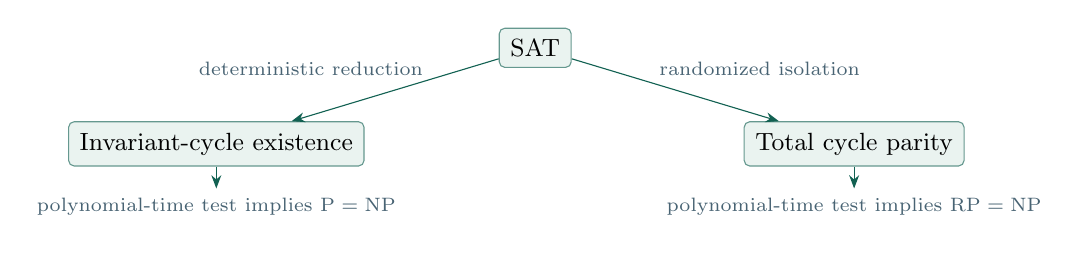
\begin{tikzpicture}[>=Stealth,box/.style={draw=pine!65,rounded corners=2pt,fill=pale,inner sep=4pt,
 align=center,font=\small},lab/.style={font=\scriptsize\color{slate},align=center}]
\node[box] (s) at (0,0) {SAT};
\node[box] (d) at (-4.05,-1.22) {Invariant-cycle existence};
\node[box] (p) at (4.05,-1.22) {Total cycle parity};
\draw[->,pine] (s)--(d); \node[lab] at (-2.85,-.27) {deterministic reduction};
\draw[->,pine] (s)--(p); \node[lab] at (2.85,-.27) {randomized isolation};
\node[lab] (dl) at (-4.05,-2.02) {polynomial-time test implies $\mathrm{P}=\mathrm{NP}$};
\node[lab] (pl) at (4.05,-2.02) {polynomial-time test implies $\mathrm{RP}=\mathrm{NP}$};
\draw[->,pine] (d)--(dl);\draw[->,pine] (p)--(pl);
\end{tikzpicture}
\end{center}
\lead{A concrete next question.} A local obstruction has been isolated for the four-clue decision problem on page 5. Does the family of perfect matchings extending the two red edges contain one that produces two opposite-side blue paths? A polynomial criterion or an NP-hardness reduction for this exact condition would advance that classification. This question and the complexity of the planar version of the cubic parity construction require separate arguments.

\hd{Historical landmarks and primary reading}
{\small
\begin{tabular}{@{}p{.11\linewidth}p{.84\linewidth}@{}}
\toprule
1971 & Cook's theorem makes satisfiability a universal target for deterministic polynomial-time NP algorithms. \citepaper{https://doi.org/10.1145/800157.805047}{The Complexity of Theorem-Proving Procedures}.\\[3pt]
1975 & Baker, Gill and Solovay gave oracle worlds with both outcomes of P versus NP. \citepaper{https://doi.org/10.1137/0204037}{Relativizations of the P =? NP Question}.\\[3pt]
1978 & Thomason's Corollaries 1.4--1.5 distinguish total and prescribed-edge Hamiltonian parity. \citepaper{https://www.dpmms.cam.ac.uk/~agt2/HC.pdf}{Hamiltonian Cycles and Uniquely Edge Colourable Graphs}.\\[3pt]
1986 & Valiant and Vazirani showed how random isolation connects SAT decision to parity-SAT. \citepaper{https://doi.org/10.1016/0304-3975(86)90135-0}{NP Is as Easy as Detecting Unique Solutions}.\\[3pt]
1990s--2010s & \citepaper{https://doi.org/10.1006/jcss.1997.1494}{Razborov--Rudich} identified the natural-proofs barrier under a hardness assumption. \citepaper{https://www.scottaaronson.com/papers/alg.pdf}{Aaronson--Wigderson} identified algebrization. \citepaper{https://people.csail.mit.edu/rrw/acc-lbs.pdf}{Williams} proved a lower bound against nonuniform ACC circuits for NEXP.\\[3pt]
2018 & Valiant, \citepaper{https://people.seas.harvard.edu/~valiant/observations-8-1-17.pdf}{Some Observations on Holographic Algorithms}, Theorems 8--9. He connects cubic Hamiltonian parity and coloring parity with color names identified, and distinguishes planar and general inputs.\\[3pt]
2023--24 & \citepaper{https://real.mtak.hu/191308/}{Hong--Mikl\'os} describe the Latin-rectangle coloring correspondence. MIT Hardness Group et al., \citepaper{https://doi.org/10.4230/LIPIcs.FUN.2024.23}{ASP-Completeness of Hamiltonicity in Grid Graphs}, Theorem 18, supplies the parsimonious starting point.\\
\bottomrule
\end{tabular}}
\smallskip
{\footnotesize The \citepaper{https://www.claymath.org/millennium/p-vs-np/}{Clay Mathematics Institute} lists P versus NP as open. The grid paper's introductory discussion of evenness requires the bipartite hypothesis for total parity. For example, $K_4$ has three Hamiltonian cycles in total, and each edge lies in two. The reduction uses its grid theorem.\par}

\pagehead{Exactly what parity queries can detect}{blackbox}
\lead{One nonlinear query.} Suppose $F$ has $k$ satisfying assignments. Fix a positive integer $b$, put $m=2^b$, and create an auxiliary Boolean formula whose witnesses are strictly increasing lists of $1$ through $m-1$ distinct models of $F$. Unused slots are fixed to zero, so each eligible subset has a unique encoding. The new formula has
\[
                 W=\sum_{j=1}^{m-1}\binom{k}{j}
                 \quad\text{models},\qquad
                 W\bmod2=\mathbf{1}\{m\nmid k\}.
\]
Indeed $(1+z)^k=\prod_{i:\,k_i=1}(1+z^{2^i})$ over $\mathbb F_2$, where $k_i$ are the binary digits of $k$. Among the coefficients indexed $0,\ldots,m-1$, precisely $2^{\operatorname{popcount}(k\bmod m)}$ are odd. Removing the constant coefficient proves the identity. An explicit CNF circuit that copies $F$ into $m-1$ slots, checks comparisons, and fixes every auxiliary variable deterministically has size polynomial in $m$ and $|F|$.

Composing this encoding with the graph reduction gives a \emph{single} cubic parity query deciding whether $2^b$ divides $k$ (negate the odd output for divisibility). If every satisfiable formula in a family has fewer than $2^b$ models, or more generally has a nonzero residue modulo $2^b$, this decides satisfiability with one parity query. It has polynomial size for $b=O(\log |F|)$. Unrestricted counts can be positive multiples of $2^b$. Fixed prime-power modular complexity and few-witness classes are classical subjects. See \citepaper{https://cis.temple.edu/~beigel/papers/bg-mods-tcs.html}{Beigel and Gill (1992)}.

\hd{Sharp bound for a procedure that sees only subset counts}
Let $S$ be an unknown subset of the $N=2^n$ assignments. Each test chooses any set $A$ and receives $|S\cap A|\bmod m$. The choice may depend on earlier answers. The exact worst-case deterministic number of tests to decide $S\ne\varnothing$ is
\[
                      \boxed{\displaystyle \left\lceil\frac{2^n}{2^b-1}\right\rceil}.
\]
For the upper bound, partition the assignments into blocks of size at most $m-1$. For the lower bound follow the all-zero transcript of $t$ tests. Write $y_x=1$ for the members of $S$. The $j$th bit of $|S\cap A|$ equals the elementary symmetric polynomial of degree $2^j$ in the bits $\{y_x:x\in A\}$ over $\mathbb F_2$, by the same coefficient identity. The indicator that all $b$ bits vanish is the product of their complements, of degree at most $m-1$. The joint zero indicator for the $t$ tests has degree at most $t(m-1)$.

The emptiness indicator has unique multilinear polynomial $\prod_x(1+y_x)$ of degree $N$. If $t(m-1)<N$, some nonempty set therefore produces the entire all-zero transcript. Restricting the argument to $t(m-1)+1$ assignments gives such a set of at most that size. A succinct CNF for this set is obtained by forbidding each missing child prefix in the binary prefix tree of its models. There are at most $n|S|$ clauses of width at most $n$. This obstruction also follows from the finite abelian $p$-group zero-sum theorem of \citepaper{https://doi.org/10.1016/0022-314X(69)90021-3}{Olson (1969)}.

\lead{Consequence for the research map.} For a polynomial-size modulus, a deterministic procedure using only these measurements still needs exponentially many in $n$. An algorithm that inspects the clauses, builds new witnesses or exploits graph structure has more information. Extending this lower bound to all deterministic algorithms would require a stronger theorem. The replication checks include 51 exact model counts and 33,874 finite families of residue tests.
\end{document}
